\documentclass[11pt]{article}

% -------------------------------------------------------------------------------- %

% *** LANGUAGE ***
%\usepackage[italian]{babel}
%\usepackage[applemac]{inputenc}

% *** PAGE LAYOUT ***
\usepackage{geometry}     
%\geometry{a4paper}                   
%\geometry{landscape}                % Activate for for rotated page geometry
%\usepackage[parfill]{parskip}       % Activate to begin paragraphs with an empty line rather than an indent

\geometry{a4paper,tmargin=2cm,bmargin=2cm,lmargin=2.5cm,rmargin=2.5cm}

% *** DEFAULT FONT SELECTION ***
\usepackage[T1]{fontenc}
\usepackage{lmodern}
\renewcommand*\familydefault{\sfdefault} %	Only if the base font of the document is to be sans serif

% *** IMAGES ***
\usepackage{graphicx}
\usepackage{subfig}


\title{
	{\Large Laboratory report 1: Challenge \\
	 \large Group 2, Tuesday Shift}
}
\author{Baron Davide, Bonetto Alessio, Mustacchi Marco, Piron Luca Vittorio}
\date{April 5, 2022}


\begin{document}

\maketitle

\section{Introduction}

	\subsection{Activity Goal}
	The goal of the challenge of this laboratory is to design a control system for QUANSER SRV-02 MOTOR such that:

	\begin{itemize}
		\item It ensures asymptotic tracking of step references;
		\item It ensures an overshoot $M_p \le 10\%$ for a 70deg step reference;
		\item It attains the minimum raise time $t_r$ you are able to achieve
	\end{itemize}

	\subsection{Model used}
	The black box $\textit{Quanser\_SRV02\_block}$ has been used in order to replace the DC motors physically present in the laboratory
	and faithfully reproduce the behaviour of the real one.

\section{Choice of control technique}

Among the possible solutions a control in state space has been chosen. 
The state space controller has been chosen instead of a PID controller because through a feedback it is possible to allocate more precisely the poles' location. \\
In order to reduce the overshoot for the step reference this controller has been modified by adding an anti windup control.
	\begin{figure}[h!]
		\centering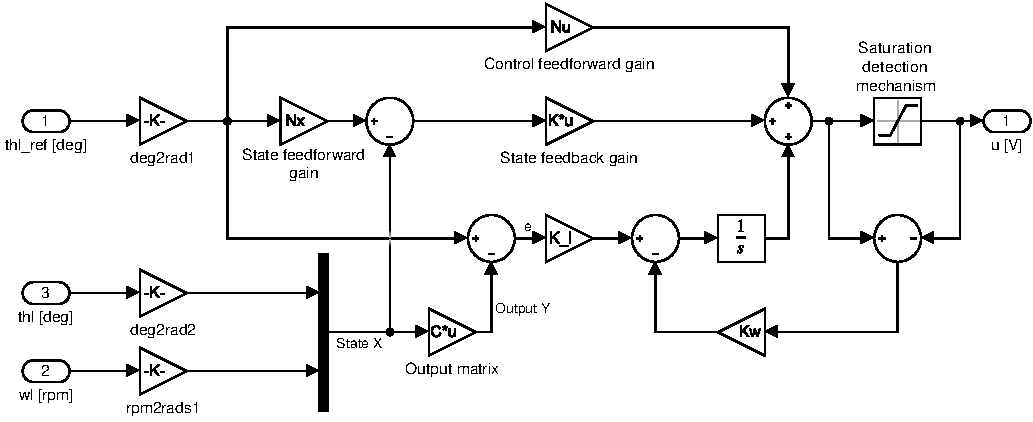
\includegraphics[scale=0.6]{images/Simulink_challenge}
		\caption{Simulink model of integral control in state space with anti windup compensation}
	\end{figure}
\vspace{-10pt}

\section{Choice of Parameters}
The choice of poles' allocation and the anti windup gain $K_w$ is made through a trial-and-error approach.\\
First of all, the poles' allocation has been chosen in order to increase the control and obtain the minimun raise time the system is able to achieve.\\
After that, the anti windup gain has been chosen in order to reduce the overshoot peak amplitude.\\
Balancing the two features, the poles and anti windup gain have been obtained:
	\begin{equation}
		\lambda_{c\{1,2\}} =-60 \pm 27.2875    \quad  \lambda_{c,3}=-80   \quad K_w = 46.25
	\end{equation} 
The poles' location imposes the control matrices K and $K_I$:
	\begin{equation}
		K = [74.2016 \:\:\:\:\:  0.8726] \quad K_I = 1849.5
	\end{equation} 


\section{Results}
The best performances that the system is able to achieve with the chosen controller are:
	\begin{equation}
		t_r = 35ms \quad M_p = 5.94\%
	\end{equation} 
    \vspace{-30pt}
	\begin{figure}[h!]
		\centering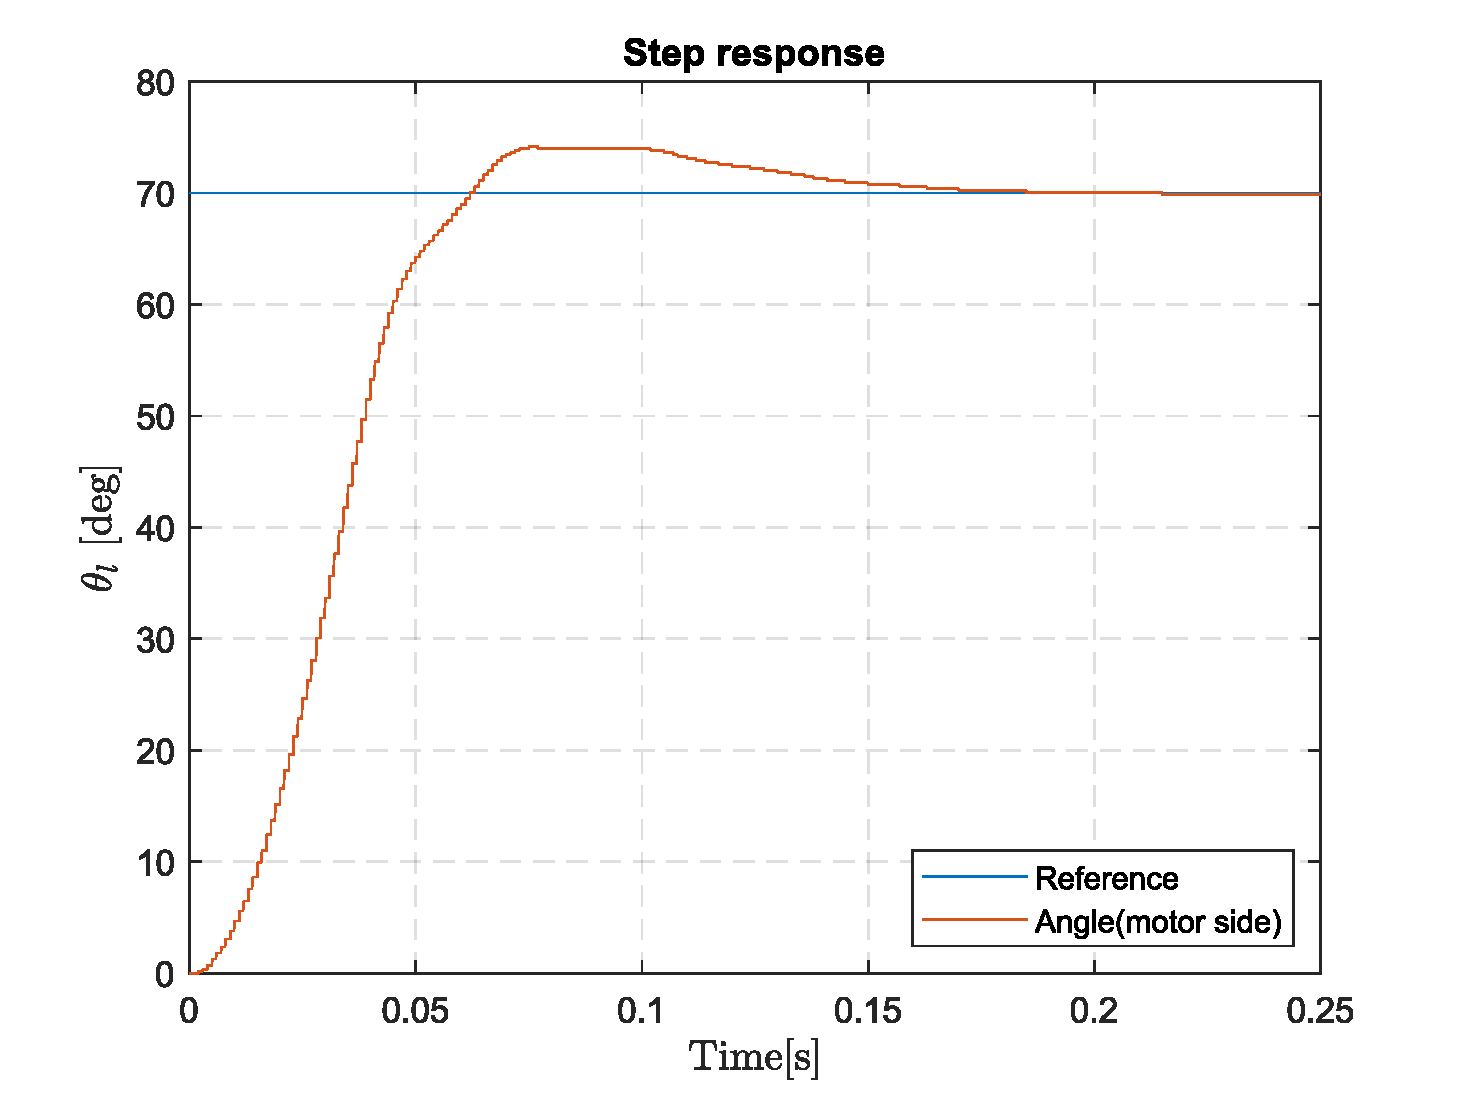
\includegraphics[scale=0.3]{images/Step_Response_Challenge}
		\vspace{-10pt}
		\caption{Step response to 70deg reference.}
	\end{figure}
\vspace{-20pt}

\section{Remarks}
A couple of observations worth highlighting were made when adjusting the controller:

	\begin{itemize}
		\item A reduced order observer should reduce the computational cost to reconstruct the state of the system, albeit the performance
			of the whole system remains substantially the same.
		\item Perhaps an LQR control should be the most efficient solution to the problem, since the trade-off between speed and
			the extent of the overshoot peak is best implemented by this type of control.
	    \item Through a parametric simulation on the poles' position it is possible to see that at a certain point the response to the step caused steady oscillations. Instead of taking the response at the limit before the oscillations, we preferred a response with a slightly higher rise time, but much smoother and with a much lower overshoot (by 3 \%).
	\end{itemize}
	
\vspace{-10pt}
	
\begin{figure}[!h]
   \begin{minipage}{0.48\textwidth}
     \centering
     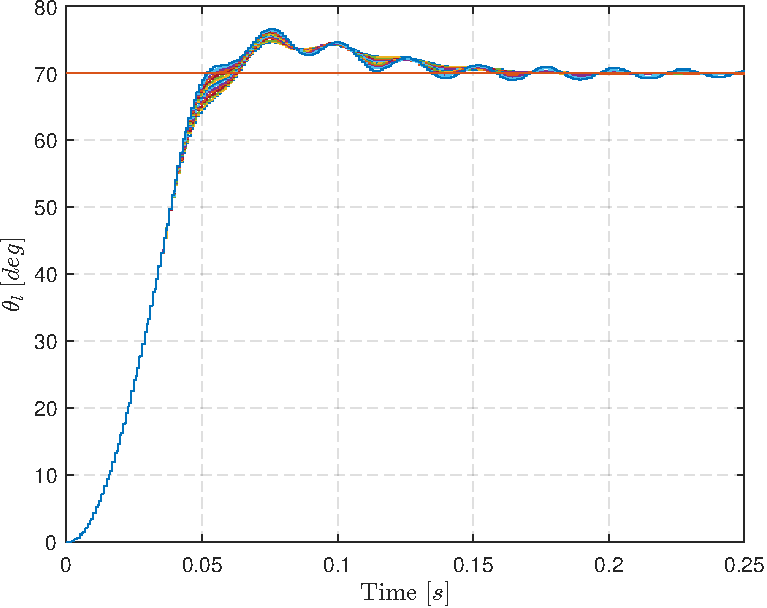
\includegraphics[width=.6\linewidth]{images/Lab1ChallengePlotParametrico.pdf}
     \caption{Parametric response}
   \end{minipage}\hfill
   \begin{minipage}{0.48\textwidth}
     \centering
     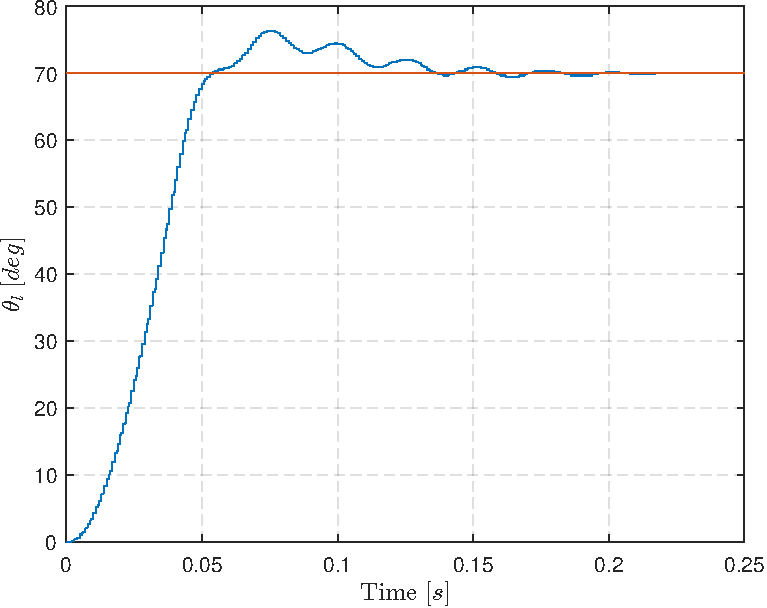
\includegraphics[width=.6\linewidth]{images/Lab1ChallengePlotScartato.pdf}
     \caption{Discarded response}
   \end{minipage}
\end{figure}
		
\end{document}

